% This file was created with tikzplotlib v0.10.1.
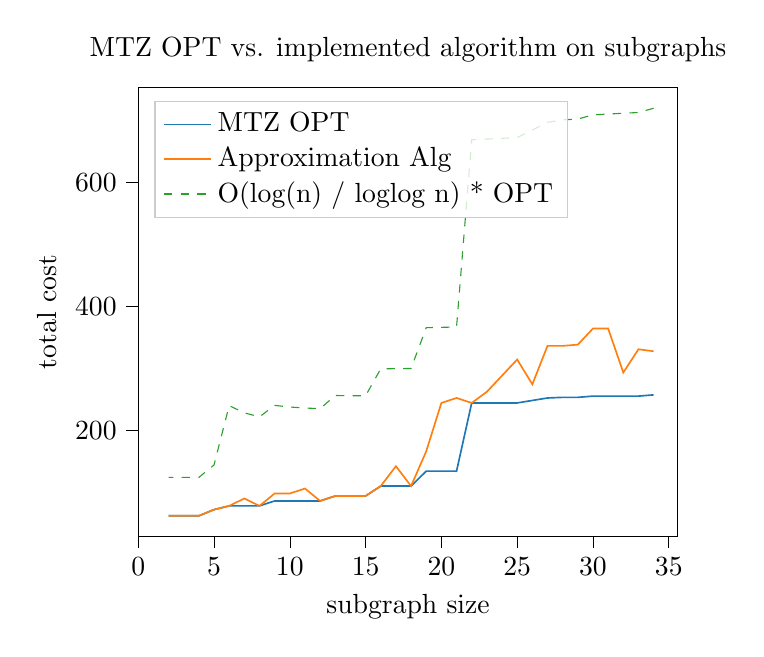
\begin{tikzpicture}

\definecolor{darkgray176}{RGB}{176,176,176}
\definecolor{darkorange25512714}{RGB}{255,127,14}
\definecolor{forestgreen4416044}{RGB}{44,160,44}
\definecolor{lightgray204}{RGB}{204,204,204}
\definecolor{steelblue31119180}{RGB}{31,119,180}

\begin{axis}[
legend cell align={left},
legend style={
  fill opacity=0.8,
  draw opacity=1,
  text opacity=1,
  at={(0.03,0.97)},
  anchor=north west,
  draw=lightgray204
},
tick align=outside,
tick pos=left,
title={MTZ OPT vs. implemented algorithm on subgraphs},
unbounded coords=jump,
x grid style={darkgray176},
xlabel={subgraph size},
xmin=0, xmax=35.6,
xtick style={color=black},
y grid style={darkgray176},
ylabel={total cost},
ymin=29.1443199994893, ymax=751.969280010724,
ytick style={color=black}
]
\addplot [semithick, steelblue31119180]
table {%
34 257
33 255
32 255
31 255
30 255
29 253
28 253
27 252
26 248
25 244
24 244
23 244
22 244
21 134
20 134
19 134
18 110
17 110
16 110
15 94
14 94
13 94
12 86
11 86
10 86
9 86
8 78
7 78
6 78
5 72
4 62
3 62
2 62
1 nan
};
\addlegendentry{MTZ OPT}
\addplot [semithick, darkorange25512714]
table {%
34 327.333333333333
33 330.5
32 293
31 364
30 364
29 338
28 336
27 336
26 274
25 314
23 262
22 244
21 252
20 244
19 166
18 110
17 142
16 110
15 94
14 94
13 94
12 86
11 106
10 98
9 98
8 78
7 90
6 78
5 72
4 62
3 62
2 62
};
\addlegendentry{Approximation Alg}
\addplot [forestgreen4416044, dashed]
table {%
34 719.113600010214
33 712.2820107532
32 711.034584554281
31 709.776360759068
30 708.50896126951
29 701.687529507932
28 700.418624777286
27 696.385230706209
26 684.089771605147
25 671.842672484082
24 670.644227518324
23 669.469217243808
22 668.328530163339
21 366.433004428298
20 365.869721883493
19 365.356178687696
18 299.552805519318
17 299.26062889844
16 299.068748775629
15 255.520313358375
14 255.632544291512
13 255.967007945437
12 234.776678508041
11 235.788960978882
10 237.427595443983
9 240.043841345742
8 221.54976130491
7 227.991880811935
6 239.639400754255
5 144
4 124
3 124
2 124
};
\addlegendentry{O(log(n) / loglog n) * OPT}
\end{axis}

\end{tikzpicture}
